\documentclass[sigplan,anonymous,review,nonacm]{acmart}
\usepackage{microtype}
\usepackage{booktabs}
\usepackage{array}
\usepackage{tabularx}
\usepackage{multirow}
\usepackage{graphicx}
\graphicspath{{results/figures/}{../results/figures/}}
\usepackage{xcolor}
\usepackage{amsmath}
\usepackage{enumitem}
\usepackage{subcaption}
\usepackage{float}
\usepackage[most]{tcolorbox}
\usepackage{tikz}
\usepackage{pgfplots}
\usepackage{balance}
\usepackage{comment}
\pgfplotsset{compat=1.18}
\usetikzlibrary{positioning,arrows.meta}

\definecolor{planred}{RGB}{180,0,0}
\definecolor{planfill}{RGB}{255,245,245}
\definecolor{darkblue}{RGB}{25,70,125}
\definecolor{darkgreen}{RGB}{25,110,70}
\hypersetup{colorlinks=true,linkcolor=darkblue,citecolor=darkgreen,urlcolor=darkblue}
\setlist{nosep,leftmargin=*}
\settopmatter{printfolios=true}

\newif\ifshowplan
\showplanfalse % Set true only in the internal planning build.
\ifshowplan
\newtcolorbox{experimentbox}[1]{
  enhanced,
  breakable,
  colback=planfill,
  colframe=planred,
  coltitle=planred,
  fonttitle=\bfseries\small,
  title={EXPERIMENT TO RUN: #1},
  boxrule=0.8pt,
  arc=1.5pt,
  left=4pt,right=4pt,top=3pt,bottom=3pt,
  before skip=5pt,after skip=5pt,
  fontupper=\small
}
\else
\excludecomment{experimentbox}
\fi

\newcommand{\tbd}{\textcolor{planred}{\textbf{TBD}}}
\newcommand{\nvml}{\textsc{NVML}}
\newcommand{\wave}{\textsc{Wave}}
\newcommand{\system}{\textsc{SensorGuard}}

\title{Beyond NVML: Sensor-Fused Hardware Telemetry for Robust AI Compute Governance}
\author{Anonymous Author(s)}
\date{}

\begin{document}

\begin{abstract}
Hardware-enabled governance requires evidence about accelerator use without inspecting model weights, data, or code. Coarse NVIDIA Management Library (NVML) telemetry is inexpensive, but adversarial workloads can approach the physical footprint of inference; per-kernel performance counters expose stronger invariants but are too expensive for continuous monitoring. We present \system{}, an architecture that combines always-on NVML with independently measured physical evidence and explicitly audits whether each sensor contributes. On a 118-run pipeline corpus drawn entirely from RTX~3090 devices, a reconstructed NVML detector identifies 22 of 23 training runs in both run-grouped and leave-one-device-out evaluation with no alerts on 95 non-training runs, yet leave-family-out evaluation identifies 0 of 23 training runs and raises 10 false alerts. The device holdout is therefore same-family interpolation, not transfer to a new GPU family. A separate RTX~3090 physical-sensor pilot contains 37 usable base-campaign runs. Reanalysis shows that the GPU rail-current clamp alone reaches 99.2\%, 100\%, and 100\% window accuracy at 15, 30, and 60~s, respectively; the motherboard clamp reaches 77.7\%, 74.5\%, and 66.4\%, and the UltraMic reaches 47.5\%, 60.6\%, and 55.1\%. Adding the microphone and motherboard channel does not improve on the GPU clamp in these grouped-by-run folds. An RTX~3090 reproduction of \wave{} matches 16/16 tight and 15/16 loose lower-bound cases, but incurs 161\% mean overhead for one NCU metric and 2,750\% for the full metric set. These are proof-of-concept and protocol-audit results, not a held-out-family fusion claim. After completing the red-box experiments, we will report the measured worst-family detection gain, false alerts per GPU-hour, time to alert, monitor overhead, and minimum retained sensor specification.
\end{abstract}
\maketitle

\section{Introduction}

Compute thresholds, licensing, and reporting regimes implicitly assume that a provider or regulator can determine whether a GPU is training a model. This is a systems question before it is a policy mechanism: a monitor must distinguish training from permitted inference and non-ML workloads, remain useful against a workload that is intentionally disguised, and do so without collecting model contents or imposing profiling-scale overhead.

Recent work establishes two complementary points. First, always-available NVML signals contain substantial information. A two-stage random-forest detector operating on nine 1~Hz signals reached 98.58\% accuracy on a 1,404-run corpus spanning 162 workloads and nine NVIDIA GPU models, with five rounds of evader-monitor iteration~\cite{rahman2026hidden}. Second, \wave{} shows that per-kernel performance counters can recover LLM architectural parameters and verify execution against analytical constraints~\cite{xu2026wave}. The two approaches occupy opposite ends of an observability continuum. NVML is inexpensive but coarse; \wave{} is structurally informative but its Nsight-based prototype reports 1,196--5,288\% collection overhead, depending on GPU and metric set.

The unresolved cases expose the research opportunity. Low-rank fine-tuning, training diluted among inference steps, low-utilization training, and a fused custom kernel that removes explicit gradient and optimizer tensors can make individual 1~Hz windows resemble inference. Aggregate AUC does not resolve whether a detector transfers to an unseen strategy at a fixed deployment threshold. Further, software telemetry requires a tamper-resistant read path and authenticated channel. These weaknesses motivate independent physical measurements, but it is unknown which sensor actually adds information after NVML, at what rate, or whether the gain justifies its cost and privacy surface.

This paper asks:

\begin{quote}
\emph{What is the smallest trusted sensor set that reliably separates training from matched inference and non-ML workloads, including previously unseen evasions, at a fixed run-level false-alert budget?}
\end{quote}

We answer this question with \system{}, a layered monitoring design and controlled sensor-selection methodology. The main evaluation fleet contains eight RTX~3090 GPUs across three hosts: seven GPUs contribute the current NVML corpus and one 200~W-capped GPU hosts the \wave{} reproduction. The completed physical-sensor pilot comes from a separate SAIGE RTX~3090 host and is analyzed with an explicit provenance boundary. Rail current is the leading external modality; thermal, RF, network, and additional acoustic measurements are retained only if they provide conditional value. NVML remains the low-cost always-on layer, while \wave{} is an offline, high-information reference rather than a deployable monitor.

The submission is organized around four auditable contributions; result claims are released only after their preregistered acceptance conditions pass:

\begin{enumerate}
  \item \textbf{A sensor-fused governance architecture.} Separately auditable modality encoders, cross-modal consistency checks, calibrated fusion, and a fixed run-level decision rule distinguish evidence from any one software stack.
  \item \textbf{A hard, matched evaluation.} A sensor-augmented roofline isolates workloads that overlap training in arithmetic intensity, throughput, utilization, and power, preventing easy clean-data examples from dominating the result.
  \item \textbf{A sensor-selection result with negative evidence.} A reproduced per-sensor ablation finds that the GPU current clamp carries the pilot's signal, while the motherboard clamp and UltraMic do not improve the combined result under the present grouped-by-run protocol.
  \item \textbf{An auditable evidence inventory.} We separate completed classifier results from collected-but-unanalyzed H200 scope and wall-power data, and from modalities for which no usable run corpus exists.
\end{enumerate}

\begin{experimentbox}{Freeze the paper claims before collecting new data}
Create a one-page preregistration containing the research questions, primary metric, false-alert budget, split policy, sensor-retention rule, and planned comparisons from Sections~\ref{sec:rq} and~\ref{sec:stats}. Hash the file and record the hash in the experiment manifest. Do not tune sensors or thresholds on the final test split. In the paper, distinguish prior published results, reproduced baselines, and new results using separate table rows.
\end{experimentbox}

\section{Scope and Threat Model}

\subsection{Governance decision}

The primary output is a run-level binary decision: \emph{training} versus \emph{not training}. ``Not training'' includes inference, scientific computing, graphics, media processing, cryptographic/mining proxies, data movement, and idle periods. Secondary labels identify inference and non-ML activity only to diagnose errors. The monitor does not claim to verify model correctness, data provenance, total training FLOPs, or compliance with a specific law.

\subsection{Adversaries}

We evaluate a tenant adversary that controls user-space code, CUDA kernels, framework configuration, scheduling, batch size, precision, power and clock requests available to the tenant, and workload interleaving. The adversary may know the feature extractor and an earlier detector, train a surrogate, and sacrifice throughput to evade detection. The adversary cannot alter the physical sensors or trusted logger in the main threat model.

A stronger hardware-operator adversary may tamper with NVML, replay traces, disconnect or occlude sensors, or alter timestamps. \system{} tests detectable forms of these attacks through cross-modal consistency and channel-health checks. It does not claim security against an operator with unrestricted physical access to every sensor and logger. A deployment for that adversary requires sealed sensor placement, device identity, secure boot, authenticated timestamps, and signed evidence. Our prototype measures the information needed by such a mechanism; it does not itself provide a production root of trust.

\subsection{Privacy boundary}

We use the term \emph{content-agnostic}, not strongly privacy-preserving. Physical traces can leak workload or model properties even without exposing weights or inputs~\cite{maia2022magnetic,arefin2025ports}. The network monitor records only timestamps, direction, packet length, and aggregate flow identifiers; it never stores payload. Cameras use fixed equipment-only regions of interest (ROIs), and raw frames are deleted after feature extraction. Section~\ref{sec:privacy} measures whether a feature set that detects training also predicts model identity or hyperparameters.

\section{Background and Related Work}

\subsection{Always-available workload telemetry}

The NeurIPS baseline samples GPU utilization, memory utilization, memory used, power, temperature, SM clock, memory clock, PCIe transmit, and PCIe receive at 1~Hz~\cite{rahman2026hidden}. From 5--60~s windows it extracts level statistics, percentiles, coefficient of variation, skew, kurtosis, autocorrelation, power-utilization ratios, PCIe totals, memory slopes and plateaus, FFT periodicity, duty cycle, and utilization transitions. Its deployed classifier is a two-stage random forest: ML versus non-ML using all features, followed by training versus inference with absolute level features removed. Grouped cross-validation prevents windows from the same run from crossing folds.

The result demonstrates that coarse physical effects are informative but also identifies two limitations that guide our design. First, subtle weight updates yield weak per-window evidence, so the current evaluation preserves the published fixed 3-of-5 run rule and measures its first causal trigger. Second, external wall power captured host-side effort that NVML omitted, motivating independent electrical sensing. A broader workload-telemetry literature likewise shows that performance counters can classify covert mining~\cite{gangwal2020mining}, and that NVML plus architectural counters captures application stress not visible in a single utilization metric~\cite{esposito2025pressure}.

\subsection{Architectural observation with \wave{}}

\wave{} fingerprints LLM inference using per-kernel compute-path and data-movement counters~\cite{xu2026wave}. It identifies nested token and layer periodicity, assigns Q/K/V/O, attention, and FFN roles, recovers model parameters, and checks structural consistency with an SMT solver. The required observations include scalar FMA/ADD/MUL counts by precision, global load/store lookup-miss sectors, and global/shared load/store instruction counts. It reports average hidden-size and FFN-dimension errors of approximately 7\% and 3\%, respectively, and average model-size error of 11\%, but current Nsight Compute collection is far too expensive for continuous monitoring.

We reproduce \wave{} for three reasons. It is a state-of-the-art hardware-observation baseline; it provides a high-information reference for whether an execution follows a transformer structure; and its counter subset supplies a target for future low-overhead hardware exposure. We do not compare its model-fingerprinting accuracy directly with training detection, because the tasks differ.

\subsection{Physical and active measurements}

Prior physical side-channel work shows that GPU power-related signals can expose workload structure~\cite{maia2022magnetic,arefin2025ports}. Timing- and memory-based active probes can reveal tensor-core contention and VRAM residency even when built-in telemetry is untrusted, although they introduce compute, memory, or power cost~\cite{monfared2026timing}. Large-scale training characterization also shows that parallelism, communication overlap, power excursions, thermal imbalance, and throttling interact in ways not summarized by arithmetic intensity alone~\cite{go2025distributed}. These results motivate measuring electrical transients, thermal dynamics, and network bursts jointly.

\subsection{Roofline and governance}

The roofline model relates throughput to arithmetic intensity and hardware ceilings~\cite{williams2009roofline}. It is valuable for characterizing bottlenecks, but it is not a classifier. In the uploaded prior sweep, 101 of 286 non-training configurations fell inside the arithmetic-intensity range of distributed training~\cite{anonymous2026always}. Differential Architecture extends roofline-style reasoning to identify hardware configurations that selectively bound targeted workloads~\cite{anonymous2026differential}. We instead condition on the overlap region and ask whether time-varying physical sensors recover class information after the roofline coordinates have become ambiguous.

\begin{table*}[t]
\centering
\caption{Positioning. ``Continuous'' means the prototype can plausibly run during an unmodified workload; it does not imply a secure readout.}
\label{tab:positioning}
\small
\begin{tabularx}{\textwidth}{p{2.45cm}Xp{2.25cm}p{3.15cm}p{4.35cm}}
\toprule
System & Primary evidence and task & Continuous / trust & Adversarial evaluation & Main limitation \\
\midrule
NVML detector~\cite{rahman2026hidden} & Nine 1~Hz management signals; training detection & Yes; software read path & 20+ workload-evasion families & Weakest on subtle custom/LoRA cases; trusted path assumed \\
\wave{}~\cite{xu2026wave} & Per-kernel PMCs; LLM inference fingerprinting & No today; privileged PMCs & Kernel split/merge transformations & 1,196--5,288\% Nsight overhead; single-GPU dense decode \\
Timing/memory probes~\cite{monfared2026timing} & Active challenges; utilization and residency & Periodic; externally checked & Untrusted host/device settings & Probe compute, memory, and power cost \\
GPU stress study~\cite{esposito2025pressure} & NVML plus CUPTI; reliability stress & Profiling; software path & Non-adversarial characterization & Not a governance detector \\
\system{} (this work) & NVML plus electrical, thermal, acoustic, RF, and network evidence; training detection & Tiered; passive modalities are independent & New unseen workload and telemetry attacks & Prototype instruments must be reduced to deployable sensor specifications \\
\bottomrule
\end{tabularx}
\end{table*}

\section{\system{} Architecture}
\label{sec:design}

\subsection{Layered observation}

Tier~0 is the nine-signal NVML stream. Tier~1 contains external passive sensors. Tier~2 is an on-demand architectural audit using the \wave{} counter subset. Each stream is timestamped, converted into modality-specific features, and scored independently. A fusion stage combines calibrated log-odds rather than concatenating all raw values. This design keeps missing sensors explicit, supports per-sensor ablation, and permits an auditor to inspect which witness caused an alert.

\subsection{Synchronization and channel health}

All host-side logs use \texttt{CLOCK\_MONOTONIC\_RAW} and record both sample and receipt timestamps. At run boundaries, a scripted load step supplies a common physical marker. Oscilloscope traces are aligned to the power edge; thermal and contact traces are aligned by cross-correlation with the slower response; acoustic and RF traces use the same scripted marker; and network timestamps are aligned to a logged Ethernet burst generated outside the measured workload. If the scopes support external triggering, one trigger is fanned out to all instruments. Otherwise, alignment error is measured rather than assumed.

Channel-health features include missing-sample fraction, timestamp drift, stuck values, clipping, impossible slopes, thermal-camera obstruction, microphone/SDR saturation, network-link or mirror loss, and disagreement between NVML power/temperature and the corresponding external modalities. A missing or unhealthy sensor is a separate state, never silently imputed as benign.

\subsection{Modality features}

Table~\ref{tab:sensors} defines the initial feature vocabulary. Features are computed over causal 1, 5, 15, 30, and 60~s windows. High-rate streams are summarized at multiple resolutions; raw samples are not fed directly into the final classifier. Each feature is normalized per physical GPU using idle and calibrated-load references collected on the same day. The final test also reports results without per-day calibration to expose operational sensitivity.

\begin{table*}[t]
\centering
\caption{Sensor roles and predeclared features. Exact device models, rates, probe placement, and calibration constants must be inserted after inventory.}
\label{tab:sensors}
\small
\begin{tabularx}{\textwidth}{p{1.7cm}p{2.2cm}Xp{3.2cm}}
\toprule
Modality & Physical quantity & Features & Hypothesized independent value \\
\midrule
NVML & Utilization, memory, power, temperature, clocks, PCIe & Earlier 166-feature vocabulary; causal windows; no future leakage & Always-on baseline and low-cost gate \\
Oscilloscope & Per-GPU 12~V input or other rated rail measurement & Mean/RMS, variance, crest factor, $dP/dt$, transient count, autocorrelation, PSD band energy, step periodicity, cross-GPU coherence, residual from NVML power & Sub-second backward/update transients and forged-NVML detection \\
Thermal camera & Spatial surface/exhaust temperature & ROI mean/max, hotspot area, spatial gradient, entropy, derivative, fitted time constant, cross-GPU imbalance & Long-run load distribution and throttling/airflow context \\
Contact temperature & Inlet, outlet, backplate, or exhaust temperature & Delta-to-inlet, slope, time constant, steady state, hysteresis & Low-cost substitute for thermal imaging \\
Ultrasound microphone & Acoustic and ultrasonic pressure near equipment & Band energy, spectral centroid/entropy, tonal peaks, modulation spectrum, transient count, coherence with electrical power & Coil/fan/controller signatures independent of software telemetry; environment-sensitive \\
RF receiver & RF emissions in preregistered bands & Band power, spectral occupancy, peak count, spectral entropy, temporal modulation, coherence with power and clocks & Independent electromagnetic activity; susceptible to ambient interference and placement \\
Mirrored Ethernet & Packet metadata from TL-SG108E mirror port, never payload & Bytes/s, packets/s, directionality, packet-size quantiles, burstiness, inter-arrival PSD, collective-like periodicity, correlation with GPU power & External data/collective phases that cross Ethernet; cannot see PCIe/NVLink \\
\wave{} PMCs & Per-kernel compute/memory events & FLOPs, off-L1 traffic, shared/global ratio, token/layer periodicity, recovered architecture & High-information reference and selective audit \\
\bottomrule
\end{tabularx}
\end{table*}

\subsection{Fusion and fixed run-level decision}

For each sensor $s$, an independently trained random forest emits a calibrated probability $p_s(t)$ for window $t$. Sensor configurations are compared on validation data, and the smallest set within one standard error of the best worst-family TPR is retained. The current paper converts the selected window probabilities into a run-level decision using the published 3-of-5 rule: an alert is raised when at least three of five consecutive windows have $p(t)\geq0.75$. The model, calibration, rule, and threshold are frozen before the held-out test is opened. Time to alert is the first causal 3-of-5 trigger; undetected runs are right-censored. A run-level alert includes the contributing modalities, channel-health state, and a hash chain over feature windows.

\subsection{Cross-modal consistency}

Physical modalities are useful even when their direct class accuracy is modest. We train regressors on benign development runs to predict external electrical power from NVML power/utilization, external temperature from NVML temperature/power history, and network bursts from distributed-job state. Residual magnitude and persistence become tamper features. Replay, scaling, offset, freezing, timestamp drift, and GPU-channel swaps should break at least one learned relation unless the adversary controls both software telemetry and the independent sensor.

\section{Research Questions and Experimental Method}
\label{sec:rq}

\subsection{Research questions}

\begin{description}[style=multiline,leftmargin=3.0cm,labelwidth=2.8cm]
\item[RQ1: Baseline fidelity.] Can the NeurIPS NVML detector and \wave{} be reproduced on RTX~3090 Ampere GPUs, and which failures arise from hardware/software version differences?
\item[RQ2: Single-sensor value.] Which physical sensor distinguishes training within the roofline-overlap and hard-evasion subsets, both alone and conditional on NVML?
\item[RQ3: Fusion and decision.] Which sensor combination maximizes worst-family run detection at a fixed false-alert budget under the fixed 3-of-5 run rule?
\item[RQ4: Hardware requirements.] How far can each stream be downsampled, quantized, spatially reduced, or duty-cycled before the gain disappears?
\item[RQ5: Robustness and privacy.] Can cross-modal checks detect telemetry manipulation, and how much model/application identity leaks from the retained features?
\end{description}

\subsection{Testbed}

The main SensorGuard fleet contains eight NVIDIA RTX~3090 GPUs across node2 (five GPUs), verifier (two GPUs), and testbed-node1 (one GPU). Its currently committed synchronized evidence is NVML/DCGM telemetry; PicoScope files in this repository are acquisition dry-runs rather than labelled workload runs. The WAVE host is separately power-capped at 200~W, while the remaining cards expose 350--370~W limits. Planned instrumentation includes three two-channel, 10~MHz Pico Technology oscilloscopes; a TOPDON TC001-A thermal camera; thermistors; an ultrasound microphone; an SDR; and mirrored Ethernet, but these planned devices are not represented as completed classifier results.

The physical proof-of-concept reported in Section~\ref{sec:physical-pilot} is a distinct June~2026 SAIGE campaign on a three-RTX~3090 node. It used an UltraMic~200K and two PicoScope~2204A oscilloscopes with clamps mapped to GPU0, GPU1, GPU2, and the motherboard rail. Workloads ran sequentially on GPU0 and the snapshot service exposed 1~Hz scalar summaries of the high-rate devices. We retain this provenance boundary: its results demonstrate physical observability, but they are not pooled with the eight-GPU SensorGuard corpus.

Because each oscilloscope has two channels, six simultaneous electrical channels may eventually be possible; headline physical results use only channels that pass probe, isolation, wiring, acquisition-rate, and synchronization checks. GPUs are characterized individually and channels are rotated where practical so GPU identity and sensor assignment are not confounded.

\begin{experimentbox}{Inventory, topology, and safety qualification}
Record: GPU UUID/SKU/VBIOS, PCIe bus and NUMA topology, any NVLink bridges, CPU, DRAM, storage, NIC, PSU, OS/kernel, NVIDIA driver, CUDA, cuDNN, NCCL, PyTorch, Nsight Compute, power/clock limits, ambient conditions, and every sensor model/firmware/rate/resolution. Draw the exact cable/mirror/probe topology. Use only manufacturer-rated isolated current probes, shunts, or instrumented power cables. Do not probe mains or exposed GPU rails without a qualified lab procedure. Measure idle noise, clipping, channel gain, timestamp jitter, and GPU-to-channel mapping. Put the resulting table in the paper and archive \texttt{nvidia-smi -q}, \texttt{nvidia-smi topo -m}, and environment-lock outputs.
\end{experimentbox}

\subsection{Workload corpus}

Table~\ref{tab:workloads} is a minimum corpus, not a menu from which easy cases may be selected after seeing results. Every class contains matched model, batch, precision, power-cap, and duration variants when applicable. Each run has a unique ID, git commit, command, seed, GPU UUIDs, start/end timestamps, sensor-health record, and useful-work measure (samples/s, tokens/s, optimizer steps/s, or application throughput).

\begin{table*}[t]
\centering
\caption{Minimum RTX~3090 evaluation matrix. Model sizes are chosen to fit 24~GB GPUs; exact versions and datasets are frozen in the manifest.}
\label{tab:workloads}
\small
\begin{tabularx}{\textwidth}{p{2.2cm}Xp{3.0cm}p{3.3cm}}
\toprule
Class & Workloads/configurations & Scaling variables & Required matched control \\
\midrule
Training & ResNet-50, BERT, GPT-2; decoder-only 1B/3B/7B full or parameter-efficient fine-tuning; DDP; FSDP/ZeRO where feasible; gradient accumulation; activation checkpointing & Batch, sequence, precision, optimizer, ranks, power cap & Same model/precision/batch inference and forward-only pass \\
Inference & Image classification; LLM prefill/decode and continuous batching; diffusion; speech-to-text & Batch, prompt/output length, concurrency, quantization & Training configuration nearest in roofline/NVML space \\
Non-ML & GEMM, FFT, SpMV/stencil, N-body, memory copy, hashing/mining proxy, Blender, video encode, network stress, idle & Problem size, duty cycle, compute/memory mix & Nearest training configuration by matched caliper \\
Evasion & Low utilization, idle dilution, memory preallocation, clock/power shaping, inference interleaving, fake collectives, frozen backbone/LoRA, training-as-inference, fused update kernel, GPU migration & Attacker budget and useful-work penalty & Non-evasive version plus matched inference \\
Telemetry attacks & Freeze, replay, offset, scale, timestamp drift, sample drop, GPU-channel swap, thermal obstruction, microphone/SDR saturation, mirror-port disconnect & Attack duration and affected channels & Unmodified synchronized trace \\
\bottomrule
\end{tabularx}
\end{table*}

\subsection{Splits and repetitions}

The unit of independence is a run, not a window. The primary final split is grouped simultaneously by physical GPU, collection day, application configuration, and evasion family. At least one GPU and one full attack family are held out from model and threshold selection. If data volume permits, we report leave-one-GPU-out, leave-one-application-family-out, and leave-one-evasion-family-out results separately. Repetitions use at least three independent starts per configuration in screening and five for the retained full evaluation. We randomize run order within thermal constraints and record cool-down state.

We use two campaigns. A fast campaign uses 180--300~s runs for electrical and NVML characterization, with other modalities included only when attached and qualified. A thermal campaign, if retained, uses a fixed warm-up, steady-state interval, and cool-down criterion based on inlet-to-device delta rather than wall-clock delay alone.

\section{Baseline Reproduction}

\subsection{NeurIPS NVML detector}

The adapted reproduction uses the same nine signals, 1~Hz sampling, a reconstructed 166-feature vocabulary, two-stage random forest, 30~s causal windows with 15~s stride, and grouped evaluation as the earlier detector~\cite{rahman2026hidden}. Because the exact original feature code is not yet in the artifact, we do not label this row a strict reproduction. The earlier 1,404-run corpus is not pooled with new physical sensor data for headline accuracy, because hardware, collection context, and missing modalities would create an easy domain cue.

\paragraph{Current pipeline diagnostic.}
The committed 118-run corpus contains 23 training and 95 non-training runs across seven physical GPUs and two collection days. Run-grouped cross-validation detects 22/23 training runs and produces 0/95 false-positive runs, with fold window AUC 0.972--0.990. These folds prevent windows from the same run crossing the split, but they do not hold out GPU, day, or application family and therefore are not headline transfer evidence. The negative exposure is only 11.45 GPU-hours: with zero events, the one-sided 95\% Poisson upper bound remains 0.262 false alerts/GPU-hour. At least 71.9 zero-event negative GPU-hours are required to place this bound below the preregistered $1/24$ GPU-hour budget.

The protocol audit in Figure~\ref{fig:generalization-audit} makes the gap concrete. Leave-one-device-out evaluation also detects 22/23 training runs with no false-positive runs, but all held-out devices are RTX~3090s; this is not a GPU-family transfer experiment. Leave-family-out evaluation detects 0/23 training runs and raises 10 false alerts among 95 non-training runs (0.873/GPU-hour). The two-day corpus cannot estimate training transfer in both directions: training examples occur only on August~25, so the fold trained on August~24 lacks the classes required by the two-stage detector. We report that fold as non-estimable rather than silently pooling days. Thus the present baseline supports device interpolation within one homogeneous GPU family, not unseen-family, unseen-workload, or temporal transfer.

\begin{figure}[t]
\centering
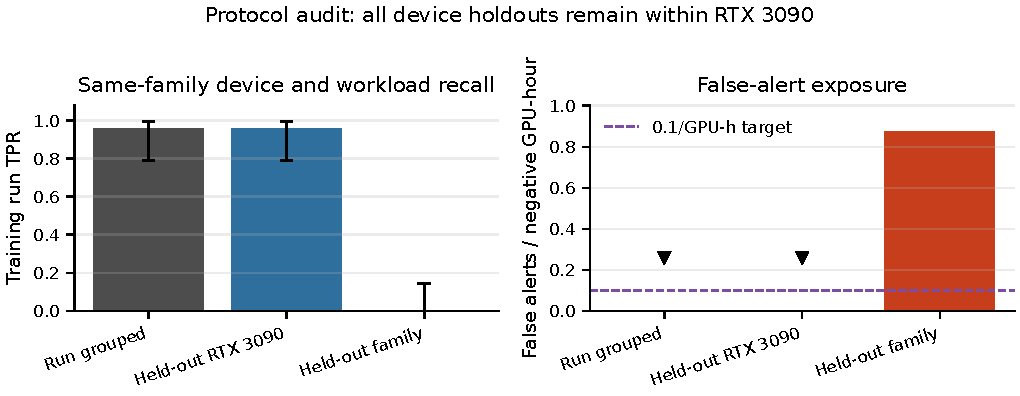
\includegraphics[width=\columnwidth]{generalization-audit.pdf}
\caption{The reconstructed baseline is sensitive to evaluation protocol. All device-held-out folds remain within the RTX~3090 family and therefore do not test cross-family transfer. Bars show aggregate run-level outcomes; TPR whiskers are Wilson 95\% intervals. Downward triangles mark one-sided 95\% false-alert-rate upper bounds when zero events were observed. Day holdout is omitted because one direction is not estimable.}
\label{fig:generalization-audit}
\end{figure}

\begin{experimentbox}{Reproduce the NVML baseline across the RTX 3090 fleet}
Run the clean core corpus first. Verify 1~Hz sample count and missingness; extract exactly the published 166 causal features; use RandomForest with 400 trees, no maximum depth, minimum leaf size 2, square-root feature sampling, and balanced classes. Report accuracy, macro-F1, ROC-AUC, PR-AUC, calibration, run-level miss rate, false alerts/GPU-hour, and time-to-first-alert under the fixed 3-of-5 rule at $\tau=0.75$. Group by run and show a per-GPU confusion matrix. Acceptance condition for a faithful reproduction: no leakage audit failures and performance uncertainty overlaps the prior result on a comparable clean subset; otherwise explain the domain shift rather than retuning on test data.
\end{experimentbox}

\subsection{\wave{} reproduction}

The RTX~3090 uses the Ampere architecture, which \wave{} did not report, although its metrics are conceptually architecture-independent. We reproduce the public artifact using GPT-2-, LLaMA-, and Qwen-style dense decoder configurations that fit 24~GB. Before running, \texttt{ncu --query-metrics} is used to map each requested metric. The required set includes scalar HFMA/FFMA/DFMA, ADD, and MUL counts; global load/store lookup-miss sectors; and global/shared load/store instruction counts. The exact names and any unavailable events are recorded.

On the 200~W-capped RTX~3090, the adapted artifact obtains 16/16 tight and 15/16 loose lower-bound decisions and 15/15 decisions for both upper-bound settings. Profiling one NCU metric adds 131--186\% runtime (161\% mean), while the WAVE metric set adds 2,254--3,059\% (2,750\% mean). Figure~\ref{fig:wave-overhead} shows all six measured decoder configurations.

\begin{figure}[t]
\centering
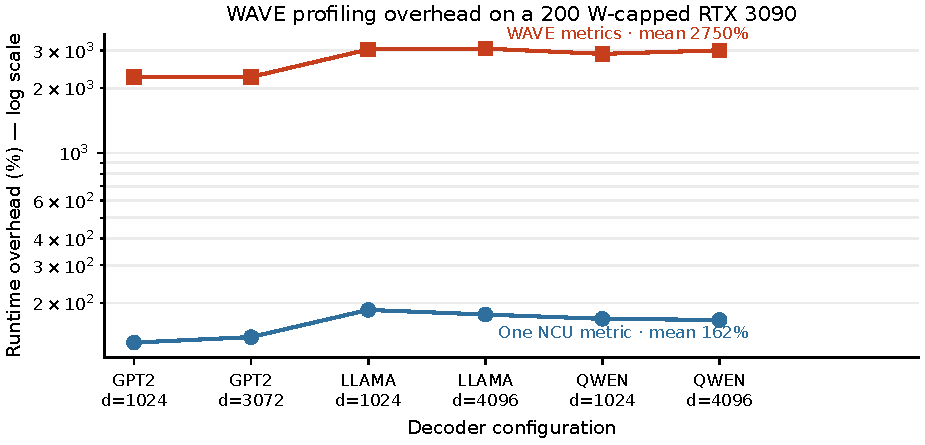
\includegraphics[width=\columnwidth]{wave-overhead.pdf}
\caption{WAVE profiling overhead on the RTX~3090 reproduction host. Values are paired against three direct executions per configuration; the y-axis is logarithmic.}
\label{fig:wave-overhead}
\end{figure}

\begin{experimentbox}{Replicate \wave{} as the architectural baseline}
Check out the public \wave{} artifact at a recorded commit and create its stated CUDA/PyTorch/Nsight environment or a containerized compatible variant. Run the authors' GPT-2, LLaMA, Qwen, and split-layer cases on the dedicated 3090 reproduction host. Measure recovered layer count, token count, batch, hidden size, FFN size, parameter-count error, lower/upper-bound false positives and negatives, solver time, trace size, and runtime slowdown. Repeat collection with each PMC family and single counters to quantify marginal overhead. Never use Nsight-profiled and unprofiled runs interchangeably in physical-sensor training. If Ampere lacks a metric, document the substitution and separately label the result ``adapted reproduction.''
\end{experimentbox}

\section{Sensor-Augmented Roofline Evaluation}
\label{sec:roofline}

\subsection{Classical roofline}

For characterization only, we obtain per-run FLOPs and DRAM bytes from Nsight Compute or analytically validated kernel counts. These profiling passes are separate from detector traces. We plot achieved FLOP/s against operational intensity (FLOPs/DRAM byte), with measured bandwidth and compute ceilings for the 3090. Training, matched inference, non-ML, and evasion configurations use distinct shapes; color does not encode the predicted label.

\subsection{Matched overlap set}

We define the training-overlap region from development data only. Each training run is paired with nearest non-training runs in standardized $[\log(\mathrm{AI}),\log(\mathrm{FLOP/s}),\overline{P}_{NVML},\overline{U}_{GPU}]$ space. The default caliper is 0.25 pooled standard deviations per coordinate; sensitivity at 0.1 and 0.5 is reported. Pair membership is frozen before sensor models are evaluated. The primary overlap-set metric is run-level TPR at the fixed global false-alert budget, accompanied by paired bootstrap confidence intervals.

\subsection{Sensor-augmented roofline}

The second roofline preserves the same axes and points but colors each point by the out-of-fold sensor-fusion log likelihood ratio. A border marks ground truth and opacity indicates calibration uncertainty. Thus the figure directly shows whether points that overlap geometrically become separable through temporal physical evidence. Separate panels show NVML only, best single external sensor, and retained fusion. A sensor does not ``solve'' overlap merely because it separates unmatched workloads elsewhere.

\begin{experimentbox}{Build both rooflines and freeze the hard subset}
For every core and adversarial configuration, run a characterization pass that records achieved FLOP/s and DRAM bytes. Validate profiler counts against analytical FLOPs for at least one kernel per family. Plot the classical roofline and report the number/fraction of non-training runs inside the training range. Construct matched pairs using the preregistered caliper, save pair IDs, and never change them after viewing sensor accuracy. Then generate the sensor-augmented roofline with strictly out-of-fold probabilities. Report overlap-set AUC/PR-AUC and TPR at the fixed false-alert budget for NVML, each sensor, NVML+sensor, and final fusion.
\end{experimentbox}

\section{Sensor Selection and Fusion Evaluation}
\label{sec:selection}

\subsection{Single-sensor screening}

\label{sec:physical-pilot}
The physical pilot provides the only completed sensor-by-sensor classifier evidence in the uploaded repositories. We downloaded the 65 committed sensor parquets from Robi Rahman's \texttt{physical-sensor-detection} branch, restricted the analysis to the original base campaign, and reproduced the branch's 99-feature combined result exactly. The evaluation uses 400-tree random forests, causal windows with approximately 50\% overlap, and five-fold \texttt{StratifiedGroupKFold} grouped by run ID. Depending on window length, 34--37 runs are long enough to contribute. Accuracy and macro F1 are window-level diagnostics; repeated workload configurations and the single instrumented host make the 100\% values optimistic.

Figure~\ref{fig:physical-ablation} is the missing per-sensor ablation. The GPU0 current clamp alone exactly matches the 99-feature electrical-plus-acoustic result at every window length. At 30~s, the GPU clamp and both-clamp configurations obtain macro F1 1.000, compared with 0.711 for the motherboard clamp and 0.509 for the UltraMic. Thus the pilot supports a narrow conclusion: GPU rail-current summaries are highly informative in this campaign, while the microphone supplies no measurable incremental accuracy. It does not establish unseen-family, unseen-host, or run-level false-alert performance.

\begin{figure*}[t]
\centering
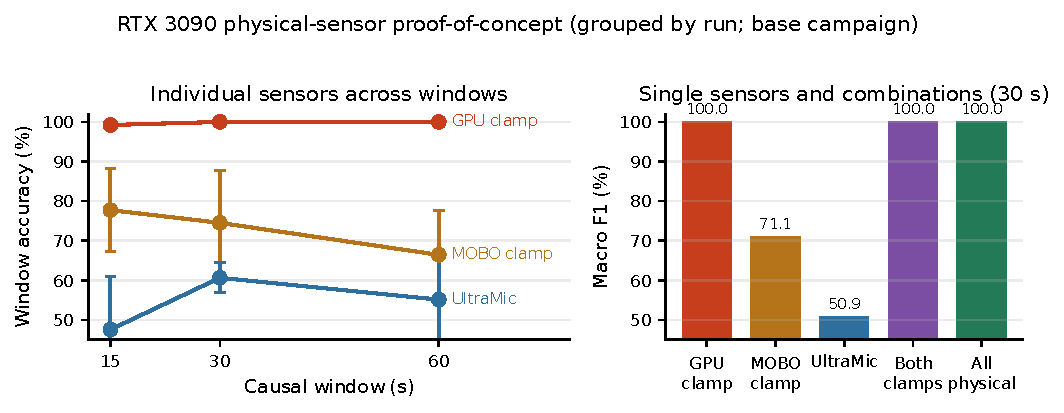
\includegraphics[width=0.94\textwidth]{physical-sensor-ablation.pdf}
\caption{Per-sensor ablation for the RTX~3090 physical pilot. The left panel shows individual sensors only, preventing the numerically identical GPU-clamp, electrical-combination, and all-physical curves from covering one another. Points are mean window accuracy across five grouped-by-run folds; whiskers show fold standard deviation, not a confidence interval. The right panel reports all individual and combined 30~s macro-F1 results.}
\label{fig:physical-ablation}
\end{figure*}

\begin{table}[t]
\centering
\caption{Thirty-second physical-sensor pilot results. Each row is a nested subset of the committed 99-feature extractor.}
\label{tab:physical-ablation}
\scriptsize
\IfFileExists{results/tables/physical-sensor-ablation.tex}{%
  % Generated by scripts/analysis/physical_sensor_ablation.py
\begin{tabular}{lrrrr}
\toprule
Sensor set & Accuracy & Macro F1 & Runs & Features \\
\midrule
GPU current clamp & 100.0\% & 1.000 & 36 & 30 \\
Motherboard clamp & 74.5\% & 0.711 & 36 & 13 \\
UltraMic & 60.6\% & 0.509 & 36 & 56 \\
Electrical clamps & 100.0\% & 1.000 & 36 & 43 \\
Electrical + acoustic & 100.0\% & 1.000 & 36 & 99 \\
\bottomrule
\end{tabular}
%
}{%
  % Generated by scripts/analysis/physical_sensor_ablation.py
\begin{tabular}{lrrrr}
\toprule
Sensor set & Accuracy & Macro F1 & Runs & Features \\
\midrule
GPU current clamp & 100.0\% & 1.000 & 36 & 30 \\
Motherboard clamp & 74.5\% & 0.711 & 36 & 13 \\
UltraMic & 60.6\% & 0.509 & 36 & 56 \\
Electrical clamps & 100.0\% & 1.000 & 36 & 43 \\
Electrical + acoustic & 100.0\% & 1.000 & 36 & 99 \\
\bottomrule
\end{tabular}
%
}
\end{table}

Figure~\ref{fig:physical-signatures} explains the current-clamp result. Mean ripple magnitude overlaps between training and non-training runs, including cuFFT, but coefficient of variation and FFT concentration expose the forward--backward--update cadence. This is also why the evidence should not be paraphrased as a generic power classifier: the clamp measures rail-current ripple, not wall watts.

\begin{figure*}[t]
\centering
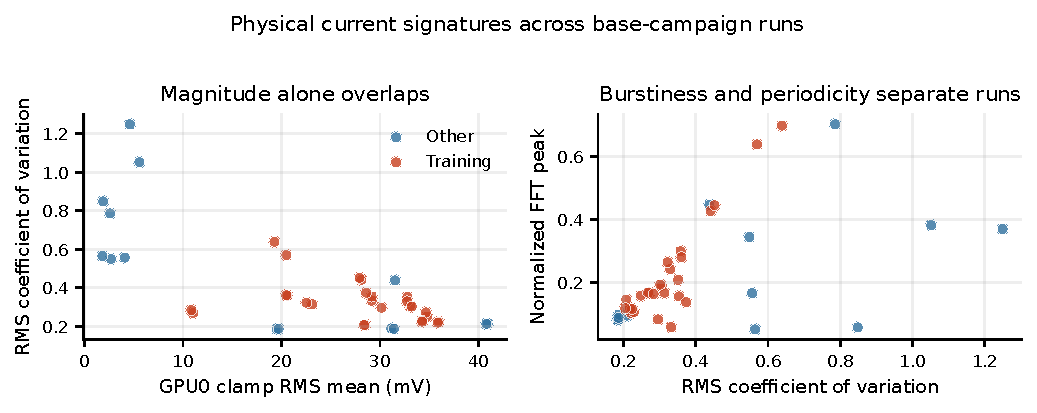
\includegraphics[width=0.94\textwidth]{physical-current-signatures.pdf}
\caption{Run-level GPU0 current-clamp summaries from the base campaign. Magnitude alone overlaps, whereas burstiness and periodicity provide additional structure. Points are runs; axes are descriptive and are not a held-out decision boundary.}
\label{fig:physical-signatures}
\end{figure*}

\begin{table*}[t]
\centering
\caption{Evidence inventory after auditing the public SensorGuard repository and all accessible branches of Robi Rahman's GPU-monitoring repository. ``Collected'' means usable files exist; it does not imply a completed detector.}
\label{tab:sensor-evidence}
\scriptsize
\begin{tabularx}{\textwidth}{p{2.1cm}p{2.4cm}p{1.8cm}Xp{2.3cm}}
\toprule
Channel & Hardware/campaign & Evidence & Quantitative result & Paper use \\
\midrule
NVML & SensorGuard RTX~3090 fleet & 118 labelled runs & 22/23 training runs detected under run- and GPU-grouped audits; leave-family-out 0/23 with 10 false alerts & Protocol audit \\
GPU rail current & SAIGE RTX~3090 pilot & 37 usable base runs & 99.2/100/100\% window accuracy at 15/30/60~s & Per-sensor proof-of-concept \\
Motherboard current & Same pilot & Same runs & 77.7/74.5/66.4\% & Negative/redundant evidence \\
UltraMic acoustic & Same pilot & Same runs & 47.5/60.6/55.1\% & Negative/redundant evidence \\
H200 electrical scope & H200~NVL, 1~kHz envelope plus raw scope snippets & 99 runs; 33 classes $\times$ 3 repetitions & Calibration $R^2=0.975$; no committed classifier output & Collected, analysis pending \\
Wall power & RTX~5080 smart-plug campaign & 49 paired workloads & Pearson $r=0.878$, $R^2=0.770$ against GPU power; no detector & Characterization only \\
Thermal/contact & SensorGuard planned instruments & No labelled run corpus found & Not estimable & Do not claim \\
RF/network & SensorGuard planned instruments & No labelled run corpus found & Not estimable & Do not claim \\
\bottomrule
\end{tabularx}
\end{table*}

Every modality is first evaluated alone, then added to the frozen NVML baseline. A sensor is judged on the hard overlap/evasion validation set, not overall clean accuracy. We report feature groups before individual feature rankings to reduce instability. The acoustic, RF, network, and thermal channels are explicitly allowed to fail; the purpose is to identify a minimum evidence set, not justify every available instrument.

\begin{experimentbox}{Calibrate and screen sensors one at a time}
For each sensor: (1) collect idle, fixed GEMM, memory-copy, and bursty-load calibration traces; (2) measure noise, drift, clipping, missingness, alignment error, and cross-GPU variability; (3) train a sensor-only classifier with grouped folds; (4) train NVML+sensor using the identical folds; (5) evaluate only on validation, including roofline-overlap and unseen-family subsets; and (6) record storage, CPU cost, setup cost, and privacy risk. Retain a sensor only if it reduces worst-family miss rate by at least 10\% relative at the same false-alert budget, the 95\% run-bootstrap interval for the improvement excludes zero, and monitoring overhead remains below 1\%. Mark sensors that fail as ruled out; do not quietly omit them.
\end{experimentbox}

\subsection{Combination search}

Sensor selection uses validation-only forward selection beginning with NVML, followed by an exhaustive check of all pairs among the retained modalities. The final set is the smallest configuration within one standard error of the best validation worst-family TPR. The test set is evaluated exactly once. We additionally report all-sensors performance and leave-one-sensor-out degradation so that a sensor selected through interaction is not mistaken for an individually strong channel.

\begin{experimentbox}{Evaluate sensor fusion without test-set selection}
Using frozen folds, compare: NVML; each sensor alone; NVML+$S_i$; best validation pair; best validation triple; all sensors; final selected set; and leave-one-out variants. Compare early feature concatenation, calibrated logistic late fusion, and boosted late fusion, but choose the deployed method on validation calibration and worst-family TPR. Report mean performance, 95\% cluster-bootstrap intervals, per-family results, calibration curves, and the cost/privacy Pareto frontier. Test the selected configuration once on held-out GPU, day, applications, and attacks.
\end{experimentbox}

\subsection{Run-level fixed detection}

Window predictions within a run are highly correlated, so an ``any-window'' rule can inflate false alerts without providing independent evidence. The current paper uses the fixed 3-of-5 rule at threshold 0.75 for continuity with the implemented baseline. Detection latency is measured from the first policy-relevant training step to the first causal 3-of-5 trigger, not from process start or warm-up; undetected runs remain right-censored.

\begin{experimentbox}{Measure fixed-rule detection of subtle weight updates}
Run matched inference, LoRA, diluted updates, and the fused custom-update kernel for durations of 1, 5, 15, 30, and 60 minutes while preserving a useful-work counter. Keep the 3-of-5 rule and probability threshold fixed. Report run TPR, false alerts/GPU-hour, median/95th-percentile time-to-first-alert, fraction detected by 1/5/15 minutes, and training throughput/energy penalty. Plot window probabilities and the first 3-of-5 trigger for representative true/false positives and the hardest miss.
\end{experimentbox}

\section{Adversarial Evaluation}

\subsection{Workload-level evasion}

The attack suite reimplements the earlier utilization, memory, mimicry, training-as-inference, multi-GPU, and white-box families, emphasizing configurations that were difficult at the operating threshold. New attacks optimize against (i) NVML only, (ii) an earlier sensor-fusion checkpoint, and (iii) a surrogate with the same feature vocabulary but different seeds. Useful training progress is always measured; an attack that stops meaningful optimization is not counted as successful evasion.

The fused custom-update kernel is central. It reorganizes backward and weight update work to remove explicit gradient tensors, optimizer kernels, and optimizer state where possible. It is paired with the same model's inference at identical batch/precision and with a forward-plus-dummy-write control. Electrical transients and memory traffic are tested as the primary discriminators.

The uploaded physical-pilot report also records three red-team rounds~\cite{rahman2026physical}. Throughput-preserving gradient accumulation, aperiodic scheduling, and gap-filling were detected. The only reported first-round evasion used a dominant steady GEMM ballast and diluted/jittered real training, but reduced useful throughput by roughly $50\times$ or more. After adding first-round attacks to training, two fresh dilution variants were reported as 100\% detected at 30~s with no false positives on the listed ResNet/GPT-2 training controls or cuFFT, N-body, mining, rendering, and idle non-training controls. Two subsequent cuFFT-mimicry rounds matched current magnitude but not the low coefficient of variation and periodicity of genuine cuFFT and were detected. These outcomes currently exist as an artifact report rather than a machine-readable result table, so we do not merge them into Figure~\ref{fig:physical-ablation} or treat them as independent test-set estimates.

\begin{table}[t]
\centering
\caption{Physical-pilot adversarial findings reported on the source branch. ``Reported'' distinguishes these narrative results from the reproduced sensor ablation.}
\label{tab:physical-redteam}
\scriptsize
\begin{tabularx}{\columnwidth}{p{1.8cm}Xp{1.55cm}}
\toprule
Round & Finding & Status \\
\midrule
1 & Reshaping attacks caught; ballast dilution evaded only with about $50\times$+ slowdown & Reported \\
Hardening & Fresh \texttt{dil\_v2/v3} caught; listed controls retained & Reported \\
2--3 & cuFFT-cover attacks matched RMS magnitude but not burstiness/periodicity; all caught & Reported \\
Multi-GPU & All-clamp code added, but collection failed and no \texttt{mg\_*} data were saved & Incomplete \\
\bottomrule
\end{tabularx}
\end{table}

\subsection{Telemetry-path attacks}

Offline perturbations apply freeze/replay, bias, scaling, clipping, missing samples, time shifts, and channel swaps to NVML. Physical channels remain unmodified. We then apply one physical-channel failure at a time to test health detection and graceful degradation. Joint compromise of all sensors is outside scope, but results show how many independent channels an attacker must control.

\begin{experimentbox}{Run sixth-round multimodal red teaming}
Freeze the first fusion detector. Give the evader its feature code and a surrogate training subset. Implement at least five new strategies, including fused-update training, power-shaping/duty-cycle optimization, acoustic/RF-noise mimicry if feasible, network-padding or suppression, and cross-GPU work migration. Hold the entire family out during defender training. Report zero-shot, after-one-round, and leave-one-family-out results at the fixed threshold, with useful-work and energy penalties. Separately inject telemetry replay/spoofing and sensor failures; report direct classification, health-alarm rate, and residual-based detection.
\end{experimentbox}

\section{Hardware Co-Design: From Instruments to a Deployable Monitor}
\label{sec:codesign}

Oscilloscopes, cameras, microphones, and SDRs establish observability but are not a production bill of materials. We therefore treat the highest-fidelity synchronized traces as a source and emulate cheaper hardware by causal filtering, downsampling, quantization, clipping, spatial ROI reduction, spectral aggregation, and duty cycling. The design output is not ``use an oscilloscope''; it is a minimum sample rate, effective number of bits, dynamic range, number and placement of thermal/contact points, acoustic/RF bands, network timestamp granularity, and local feature-compute/storage budget.

For electrical sensing, candidate rates are logarithmically spaced from the maximum reliable acquisition rate down to 1~Hz; bit depths include 16, 12, 10, 8, 6, and 4 effective bits. For thermal sensing, we sweep frame rate and replace images with progressively smaller ROI statistics. For ultrasound and RF, we reduce sample rate/bandwidth and aggregate frequency bins. For mirrored Ethernet, we coarsen timestamps and aggregate packet sizes into bins. For \wave{}, we evaluate counter-family subsets and sampling only selected kernels/windows. All transformations are performed within each training fold to avoid using future samples or test normalization.

\begin{experimentbox}{Derive minimum sensor specifications}
Starting from raw retained-sensor traces, sweep sample rate, anti-alias filter, quantization, dynamic range, ROI resolution, timestamp granularity, and duty cycle. Recompute features and retrain under identical grouped folds. For each design point report worst-family TPR at the fixed false-alert budget, latency, bytes/GPU-hour, logger CPU utilization, and estimated acquisition duty. Select the lowest-cost point within one standard error of full-fidelity performance. Confirm the chosen point with a small hardware-in-the-loop rerun rather than relying only on offline degradation.
\end{experimentbox}

\section{Privacy, Overhead, and Trust Evaluation}
\label{sec:privacy}

\subsection{Privacy leakage}

Content-agnostic does not mean identity-free. We train attacker probes to infer application family, model family, model size bin, batch-size bin, and precision from each feature set. The desired representation lies on a utility-privacy frontier: high training-detection TPR but low sensitive-attribute accuracy. We compare raw features, locally aggregated features, rate/bit-depth reduction, feature clipping, and calibrated noise. We do not claim differential privacy unless a formal mechanism and privacy budget are implemented.

\subsection{Runtime and operational overhead}

Passive sensing should not slow the GPU, but logging, timestamping, image processing, network capture, and classifier inference consume host resources and I/O. We measure workload throughput with no monitor, NVML only, each sensor logger, final fusion, and \wave{} profiling. We report CPU utilization, memory, storage/network logging rate, energy, and any GPU throughput change. Scope probes are also checked for electrical perturbation within instrument accuracy.

\subsection{Trust and evidence integrity}

The prototype creates a per-run manifest and hash chain over feature windows. A deployment should bind GPU identity, sensor-channel identity, timestamps, classifier version, and alert to a device-held key. We evaluate replay and channel-swap detection, but do not equate a software hash chain with hardware attestation.

\begin{experimentbox}{Measure privacy, overhead, and evidence integrity}
Run sensitive-attribute probes with exactly the same grouped splits as the detector. Plot training utility versus model/application inference accuracy for each aggregation and degradation setting. Measure throughput and host overhead with randomized A/B order and at least five repetitions per representative workload. Verify no payloads or human images are retained. Test hash-chain verification, dropped/reordered windows, trace replay, GPU UUID/channel swap, and clock drift. Report limitations of the software prototype and list the root-of-trust functions required in production.
\end{experimentbox}

\section{Metrics and Statistical Analysis}
\label{sec:stats}

The primary endpoint is the minimum TPR across preregistered evasion families at a run-level false-alert budget of 0.1/GPU-hour. We also report a stricter 0.01/GPU-hour point. Secondary metrics are ROC-AUC, PR-AUC, expected calibration error, missed-run rate, time-to-first-alert, clean accuracy, and application throughput/energy. Window-level metrics are diagnostic only.

Confidence intervals use a hierarchical bootstrap: sample workload families, then runs, preserving all windows and modalities within a run. Sensor improvements are paired on identical runs. We report the 95\% interval for $\Delta$TPR and relative miss reduction. Multiple sensor comparisons use Holm correction. Hyperparameters, thresholds, sensor selection, and stopping rules use development/validation data only. Missing channels are evaluated both as failures and through the system's explicit health state; runs are not deleted merely because a sensor performed poorly.

\begin{table}[t]
\centering
\caption{Completed audits and pilot results. Metrics are not directly interchangeable: NVML rows are run-level, the physical pilot is window-level, and \wave{} performs architectural verification rather than training detection.}
\label{tab:primary}
\scriptsize
\begin{tabularx}{\columnwidth}{Xcccc}
\toprule
Monitor & Worst TPR & FA/GPU-h & Alert p50 & Ovh. \\
\midrule
NVML run-grouped diagnostic & 22/23 & 0 observed$^*$ & N/A & Not measured \\
NVML leave-device-out (RTX~3090) & 22/23 & 0 observed$^*$ & N/A & Not measured \\
NVML leave-family-out audit & 0/23 & 0.873 & N/A & Not measured \\
GPU clamp pilot (30~s)$^\dagger$ & 1.000 acc. & N/A & N/A & Passive \\
Motherboard clamp pilot$^\dagger$ & 0.745 acc. & N/A & N/A & Passive \\
UltraMic pilot$^\dagger$ & 0.606 acc. & N/A & N/A & Passive \\
\wave{} (different task) & N/A & N/A & N/A & 2,750\% \\
\bottomrule
\end{tabularx}
\parbox{\columnwidth}{\scriptsize $^*$11.45 negative GPU-hours; one-sided 95\% zero-event upper bound is 0.262 false alerts/GPU-hour. $^\dagger$Mean grouped-fold window accuracy on 36 runs long enough for a 30~s window, not run TPR.}
\end{table}

\section{Sensor-Retention Decision Logic}

High-rate electrical sensing is the primary candidate because it directly tests whether weight writes and backward phases produce transient structure hidden by 1~Hz averaging. Contact temperature, thermal imaging, mirrored Ethernet, ultrasound, and RF remain optional: each must demonstrate conditional value beyond NVML and electrical evidence under placement/day shifts. The network channel is interpreted only when relevant traffic crosses the monitored switch; it cannot observe intra-node PCIe or NVLink.

A negative result is useful: ruling out redundant modalities narrows the deployable sensor set. The central outcome is the cost--robustness frontier, not the largest possible classifier. Modalities failing the preregistered retention rule remain in the ruled-out-sensor table rather than disappearing from the evaluation.

\section{Discussion}

\subsection{Why this is an architecture paper}

The work is not only an application of multimodal machine learning. It evaluates the observability contract a governable accelerator must expose: which physical invariants are useful, at what temporal/spatial resolution, how independent channels detect telemetry tampering, and when an expensive architectural audit should be triggered. The downsampling and counter-subset experiments translate empirical traces into hardware interface requirements. The adaptive tiering separates cheap continuous monitoring from selective fine-grained verification.

\subsection{Relationship to prior submissions}

The NeurIPS work contributes the NVML corpus, adversarial iteration method, and evidence that coarse telemetry detects training~\cite{rahman2026hidden}. The earlier roofline study contributes the observation that non-training workloads overlap training in arithmetic-intensity space~\cite{anonymous2026always}. The SAIGE physical campaign was uploaded separately and is included here as a clearly labelled pilot rather than silently presented as SensorGuard's final held-out experiment~\cite{rahman2026physical}. If venue policies treat any prior manuscript or artifact as concurrent or substantially overlapping, the authors must disclose it and narrow duplicated text/results before submission.

\subsection{Limitations}

The physical classifier evidence comes from one three-RTX~3090 host, one active GPU, approximately two repetitions per base workload, and grouped window evaluation. It may encode host, channel, or workload-family regularities and must not be read as a 100\% deployment result. The H200 corpus offers a valuable cross-architecture electrical dataset, but no classifier output has yet been committed. RTX~3090 results may not transfer to H100/H200/B200 power delivery, HBM, NVLink/NVSwitch, cooling, or confidential-computing modes. Thermal, contact, RF, and network modalities remain unevaluated. The monitor detects training-like physical behavior, not intent or legal noncompliance, and an adaptive adversary may discover a new joint evasion.

\section{Conclusion}

\system{} combines always-on NVML with independent physical evidence, but the audit shows why modality claims must be separated by protocol and provenance. NVML interpolates across the current homogeneous GPU fleet yet fails the leave-family-out audit. In the separate physical pilot, a GPU current clamp is sufficient to reproduce the combined classifier, while the motherboard clamp and UltraMic add no measured accuracy. The next decisive experiment is therefore not a larger multimodal model: it is a run-level, held-out-family validation of rail-current sensing across hosts and architectures, beginning with the already collected H200 corpus.

\ifshowplan
\appendix
\onecolumn
\section{How Prior NeurIPS Data Determines Sensor Tests}
\label{app:prior}

Table~\ref{tab:prior-map} makes the provenance and decision logic explicit. Values in the first four rows come from the uploaded NeurIPS manuscript; the custom-kernel observations come from the subsequent author-response extension and must be labeled non-archival unless incorporated into a released revision. No physical sensor result is inferred from these data.

\begin{table}[H]
\centering
\caption{Prior evidence used to choose, add, or rule out sensors. ``Action'' is a test decision, not a claimed outcome.}
\label{tab:prior-map}
\small
\begin{tabularx}{\textwidth}{p{3.0cm}p{3.2cm}Xp{3.7cm}}
\toprule
Prior observation & Exact prior data used & Implication & New sensor action/test \\
\midrule
Strong aggregate NVML baseline & 1,404 runs; 162 workloads; about 117 GPU-hours; 867 training, 352 inference, 185 other; nine 1~Hz signals; 26,496 30~s windows & New work must target errors and transfer, not repeat clean random splits & Freeze NVML as baseline; optimize worst-family run TPR and false alerts/GPU-hour \\
Hard subtle updates & Held-out white-box/low-utilization families show high AUC but low alert rate at the original threshold; 7B white-box LoRA was particularly difficult in the response & Evidence exists but is weak per window & Test high-rate rail power and power-NVML residuals under the fixed 3-of-5 rule \\
Highly correlated windows & Reported score correlation remains about 0.98--0.99 from 30~s to hours in the response analysis & Repeated voting may not create independent information & Report first-trigger latency and false alerts for 3-of-5 using full runs \\
External power adds host information & 49-workload smart-plug subset; wall and NVML power strongly correlated, with workload-dependent residuals & Independent electrical sensing may reveal host or fast transient costs hidden by NVML & Prioritize oscilloscope; quantify residual and rate/bit-depth requirement \\
Custom fused update & Response extension expanded to 1,727 runs, including 38 runs from five custom-kernel workloads; prior classifier had very low zero-shot detection and only partial run recovery after retraining & A kernel can minimize explicit training artifacts but must still write weights & Make fused-update kernel the primary held-out attack; pair with identical inference and dummy-write controls \\
Multi-GPU training was already easy in NVML corpus & Earlier multi-GPU evasion was detected strongly on datacenter nodes & Network sensing may be redundant unless it exposes a new trust domain & Retain mirrored Ethernet only if conditional gain appears; distinguish intra-node from observed external traffic \\
Roofline overlap & Prior sweep: 101/286 non-training configurations inside training arithmetic-intensity range & Utilization/AI alone are not a valid detector & Freeze a matched overlap set and color the second roofline by out-of-fold sensor evidence \\
Temperature/power vary with parallelism & Distributed-training characterization reports power excursions, thermal imbalance, and compute-communication effects~\cite{go2025distributed} & Slow modalities may help long distributed runs but are environment-sensitive & Test thermal/contact sensors under randomized placement/day and report cross-environment transfer \\
\bottomrule
\end{tabularx}
\end{table}

\section{Detailed End-to-End Experiment Procedure}
\label{app:steps}

\subsection{A. Freeze code, environment, and labels}

\begin{enumerate}
\item Create immutable IDs for workload, run, GPU UUID, sensor channel, day, seed, and git commit.
\item Store commands and labels before execution. A training label requires at least one optimizer/weight-update step and a useful-work counter.
\item Freeze development, validation, and test groups before sensor selection. Store only split IDs, not derived windows, in the split file.
\item Save software versions, container digest, compiler flags, environment variables, power/clock state, and topology outputs.
\item Define failure policies: OOM, thermal throttling, sensor clipping, logger crash, and alignment failure. Failed runs remain in an audit table even if excluded by a preregistered rule.
\end{enumerate}

\subsection{B. Establish sensor timing and calibration}

\begin{enumerate}
\item Map each GPU UUID to PCIe slot, power cable, scope channel, thermal-camera ROI, contact sensor, microphone placement, SDR placement/band, and any observable network flow.
\item With the GPU idle, collect at least ten minutes to estimate baseline noise and drift.
\item Run fixed-duration GEMM, memory-copy, and alternating 5~s load/idle steps. Use the edge sequence to estimate alignment and response time.
\item Repeat on every GPU/channel permutation. If practical, rotate scopes across GPUs to separate sensor-channel effects from GPU effects.
\item Set acquisition range from calibration only. Re-run clipped channels; never normalize clipping away.
\item Record ambient inlet temperature and cooling/fan policy. Begin thermal runs only within the preregistered starting-temperature band.
\end{enumerate}

\subsection{C. Collect clean and matched workloads}

\begin{enumerate}
\item Run clean training, matched inference, and non-ML workloads in randomized blocks.
\item For each configuration, collect an unprofiled synchronized sensor run and a separate Nsight characterization run.
\item Compute useful work and energy. Confirm that class labels and progress counters are nonzero.
\item Build the classical roofline and matched overlap set from development characterization only.
\item Audit that no window from a run, checkpoint, or repeated trace crosses groups.
\end{enumerate}

\subsection{D. Reproduce baselines}

\begin{enumerate}
\item Run the strict NVML pipeline with published features/hyperparameters and causal windows.
\item Freeze the prior 3-of-5 rule and its 0.75 probability threshold before the held-out evaluation.
\item Query 3090 PMC availability and run \wave{} at a pinned artifact commit. Save raw reports and solver outputs.
\item Compare \wave{} structural recovery and overhead with the published 4090/5080/H100 results, explicitly labeling hardware differences.
\end{enumerate}

\subsection{E. Screen sensors}

\begin{enumerate}
\item Extract only the preregistered features in Table~\ref{tab:sensors}.
\item Evaluate each modality alone and NVML plus that modality with identical grouped folds.
\item Inspect conditional gain on roofline-overlap, LoRA/dilution, fused-update, and benign high-utilization subsets.
\item Apply the retention rule. Keep a public table of accepted and rejected sensors with confidence intervals and costs.
\end{enumerate}

\subsection{F. Fuse and red-team}

\begin{enumerate}
\item Select the smallest validation sensor set within one standard error of the best worst-family TPR.
\item Freeze the random-forest fusion model, calibration, 3-of-5 rule, and threshold.
\item Give the frozen feature code to the attack author and collect new evasion families without retraining the detector.
\item Evaluate zero-shot on the untouched test set; only then run one defender update and report it separately.
\item Inject telemetry and sensor-health attacks, one channel and multiple channels at a time.
\end{enumerate}

\subsection{G. Derive hardware requirements}

\begin{enumerate}
\item Causally low-pass and downsample raw signals; avoid aliasing.
\item Quantize after fixing range from training calibration. Never use test extrema.
\item Reduce camera data to ROIs and scalar/spatial features; delete raw frames according to the data plan.
\item Measure detection, data rate, logger cost, and privacy leakage at every design point.
\item Rerun a representative workload subset using the selected acquisition settings to validate the offline emulation.
\end{enumerate}

\subsection{H. Produce paper tables and figures}

\begin{enumerate}
\item Table: full testbed and sensor specifications.
\item Figure: timeline-aligned example traces for matched inference, ordinary training, and fused-update training.
\item Figure: classical and sensor-augmented rooflines.
\item Figure: worst-family TPR versus false alerts/GPU-hour and time-to-alert.
\item Figure: sensor cost/privacy/robustness Pareto frontier.
\item Figure: sample-rate/bit-depth heat map with selected hardware point.
\item Table: add-one and leave-one-out sensor ablation.
\item Table: per-attack zero-shot detection and useful-work penalty.
\item Table: privacy probes and monitor overhead.
\end{enumerate}

\section{Reproduction Checklist for \wave{}}

\begin{enumerate}
\item Use the public artifact URL reported by \wave{}: \url{https://github.com/sept-usc/Wave}. Pin the commit and preserve its license notice.
\item Record whether the original CUDA~12.8, PyTorch~2.7.0, and Nsight Compute~2025.1+ environment can be reproduced exactly on the RTX~3090 driver. If not, record every change.
\item Query and save the concrete metric names for scalar half/single/double FMA, ADD, MUL; global load/store lookup-miss sectors; and global/shared load/store instruction counts. The paper notes that names may vary by toolkit.
\item Preserve a 32-byte L1/TEX sector assumption only after confirming it for the collected metric.
\item Reproduce token/layer periodicity, role assignment, direct parameter recovery, SMT lower/upper-bound tests, split-layer attacks, and overhead.
\item Report missing metrics and unsupported configurations; do not silently replace them with elapsed time or NVML counters.
\end{enumerate}

\section{Result Templates}

\begin{table}[H]
\centering
\caption{Sensor ablation template. Fill with paired run-level results and 95\% confidence intervals.}
\small
\begin{tabular}{lcccccc}
\toprule
Configuration & Clean TPR & Overlap TPR & Worst-family TPR & FA/GPU-h & Alert p50 & Bytes/GPU-h \\
\midrule
NVML & \tbd & \tbd & \tbd & \tbd & \tbd & \tbd \\
Power only & \tbd & \tbd & \tbd & \tbd & \tbd & \tbd \\
Thermal only & \tbd & \tbd & \tbd & \tbd & \tbd & \tbd \\
Contact temperature only & \tbd & \tbd & \tbd & \tbd & \tbd & \tbd \\
Visible ROI only & \tbd & \tbd & \tbd & \tbd & \tbd & \tbd \\
Network metadata only & \tbd & \tbd & \tbd & \tbd & \tbd & \tbd \\
NVML + each accepted sensor & \tbd & \tbd & \tbd & \tbd & \tbd & \tbd \\
Selected fusion & \tbd & \tbd & \tbd & \tbd & \tbd & \tbd \\
\bottomrule
\end{tabular}
\end{table}

\begin{table}[H]
\centering
\caption{Attack template. ``Progress'' is useful training progress relative to the corresponding non-evasive run.}
\small
\begin{tabular}{lcccccc}
\toprule
Held-out family & Runs & NVML TPR & Fusion TPR & Health/tamper TPR & Progress & Energy/progress \\
\midrule
Low utilization & \tbd & \tbd & \tbd & N/A & \tbd & \tbd \\
White-box LoRA & \tbd & \tbd & \tbd & N/A & \tbd & \tbd \\
Diluted training & \tbd & \tbd & \tbd & N/A & \tbd & \tbd \\
Fused update kernel & \tbd & \tbd & \tbd & N/A & \tbd & \tbd \\
Cross-GPU migration & \tbd & \tbd & \tbd & N/A & \tbd & \tbd \\
NVML replay/freeze & \tbd & \tbd & \tbd & \tbd & N/A & N/A \\
Sensor disconnect/occlusion & \tbd & \tbd & \tbd & \tbd & N/A & N/A \\
\bottomrule
\end{tabular}
\end{table}

\twocolumn
\fi
\begin{thebibliography}{99}
\small

\bibitem{rahman2026hidden}
R. Rahman and S. Tajdari. Detecting Hidden ML Training With Zero-Overhead Telemetry. NeurIPS 2026 submission and author-response materials, 2026.

\bibitem{xu2026wave}
H. Xu, C. Gong, B. Liu, H. Zheng, B. Chen, and M. Li. Wave: Leveraging Architecture Observation for Privacy-Preserving Model Oversight. In \emph{ASPLOS}, 2026. DOI: \href{https://doi.org/10.1145/3779212.3790247}{10.1145/3779212.3790247}.

\bibitem{williams2009roofline}
S. Williams, A. Waterman, and D. Patterson. Roofline: An Insightful Visual Performance Model for Multicore Architectures. \emph{Communications of the ACM}, 52(4):65--76, 2009.

\bibitem{shavit2023chinchilla}
Y. Shavit. What Does It Take to Catch a Chinchilla? Verifying Rules on Large-Scale Neural Network Training via Compute Monitoring. arXiv:2303.11341, 2023.

\bibitem{ogara2025hem}
A. O'Gara, G. Kulp, W. Hodgkins, J. Petrie, V. Immler, A. Aysu, K. Basu, S. Bhasin, S. Picek, and A. Srivastava. Hardware-Enabled Mechanisms for Verifying Responsible AI Development. arXiv:2505.03742, 2025.

\bibitem{monfared2026timing}
S. K. Monfared, F. Ganji, D. Holcomb, and S. Tajik. Timing and Memory Telemetry on GPUs for AI Governance. arXiv:2602.09369, 2026.

\bibitem{esposito2025pressure}
G. Esposito, J.-D. Guerrero-Balaguera, J. E. Rodriguez Condia, M. Sonza Reorda, M. Barbiero, and R. Fortuna. GPU Under Pressure: Estimating Application's Stress via Telemetry and Performance Counters. arXiv:2511.05067, 2025.

\bibitem{go2025distributed}
S. Go, J. Park, S. More, H. Wu, I. Wang, A. Jezghani, T. Krishna, and D. Mahajan. Characterizing the Efficiency of Distributed Training: A Power, Performance, and Thermal Perspective. In \emph{MICRO}, 2025. DOI: \href{https://doi.org/10.1145/3725843.3756111}{10.1145/3725843.3756111}.

\bibitem{gangwal2020mining}
A. Gangwal, S. G. Piazzetta, G. Lain, and M. Conti. Detecting Covert Cryptomining Using HPC. In \emph{CANS}, 2020.

\bibitem{maia2022magnetic}
H. T. Maia, C. Xiao, D. Li, E. Grinspun, and C. Zheng. Can One Hear the Shape of a Neural Network? Snooping the GPU via Magnetic Side Channel. In \emph{USENIX Security}, 2022.

\bibitem{arefin2025ports}
S. E. Arefin and A. Serwadda. Exploiting HDMI and USB Ports for GPU Side-Channel Insights. In \emph{CODASPY}, 2025.

\bibitem{anonymous2026differential}
Anonymous. Differential Architecture: Limiting Performance of Targeted Applications. ISCA submission, 2026.

\bibitem{anonymous2026always}
Anonymous. Classifying GPU Workloads via Always-Available Telemetry for AI Compute Governance. Manuscript, 2026.

\bibitem{rahman2026physical}
R. Rahman. Physical-Sensor Workload Detection and Adversarial Red-Teaming. GPU-monitoring artifact, branch \texttt{physical-sensor-detection}, commits \texttt{0b3c69f} and \texttt{baf6108}, 2026. \url{https://github.com/robirahman/GPU-monitoring/tree/physical-sensor-detection}.

\bibitem{tang2022supercloud}
B. J. Tang et al. The MIT Supercloud Workload Classification Challenge. In \emph{IPDPSW}, 2022.

\bibitem{almusaddar2026shadowscope}
G. Almusaddar, Y. Zhang, S. Ganjisaffar, B. Williams, Y. D. Liu, D. Ponomarev, and N. Abu-Ghazaleh. ShadowScope: GPU Monitoring and Validation via Composable Side Channel Signals. In \emph{ASPLOS}, 2026.

\end{thebibliography}

\end{document}
